% Options for packages loaded elsewhere
\PassOptionsToPackage{unicode}{hyperref}
\PassOptionsToPackage{hyphens}{url}
\documentclass[
  english,
  man,floatsintext]{apa6}
\usepackage{xcolor}
\usepackage{amsmath,amssymb}
\setcounter{secnumdepth}{-\maxdimen} % remove section numbering
\usepackage{iftex}
\ifPDFTeX
  \usepackage[T1]{fontenc}
  \usepackage[utf8]{inputenc}
  \usepackage{textcomp} % provide euro and other symbols
\else % if luatex or xetex
  \usepackage{unicode-math} % this also loads fontspec
  \defaultfontfeatures{Scale=MatchLowercase}
  \defaultfontfeatures[\rmfamily]{Ligatures=TeX,Scale=1}
\fi
\usepackage{lmodern}
\ifPDFTeX\else
  % xetex/luatex font selection
\fi
% Use upquote if available, for straight quotes in verbatim environments
\IfFileExists{upquote.sty}{\usepackage{upquote}}{}
\IfFileExists{microtype.sty}{% use microtype if available
  \usepackage[]{microtype}
  \UseMicrotypeSet[protrusion]{basicmath} % disable protrusion for tt fonts
}{}
\makeatletter
\@ifundefined{KOMAClassName}{% if non-KOMA class
  \IfFileExists{parskip.sty}{%
    \usepackage{parskip}
  }{% else
    \setlength{\parindent}{0pt}
    \setlength{\parskip}{6pt plus 2pt minus 1pt}}
}{% if KOMA class
  \KOMAoptions{parskip=half}}
\makeatother
% Make \paragraph and \subparagraph free-standing
\makeatletter
\ifx\paragraph\undefined\else
  \let\oldparagraph\paragraph
  \renewcommand{\paragraph}{
    \@ifstar
      \xxxParagraphStar
      \xxxParagraphNoStar
  }
  \newcommand{\xxxParagraphStar}[1]{\oldparagraph*{#1}\mbox{}}
  \newcommand{\xxxParagraphNoStar}[1]{\oldparagraph{#1}\mbox{}}
\fi
\ifx\subparagraph\undefined\else
  \let\oldsubparagraph\subparagraph
  \renewcommand{\subparagraph}{
    \@ifstar
      \xxxSubParagraphStar
      \xxxSubParagraphNoStar
  }
  \newcommand{\xxxSubParagraphStar}[1]{\oldsubparagraph*{#1}\mbox{}}
  \newcommand{\xxxSubParagraphNoStar}[1]{\oldsubparagraph{#1}\mbox{}}
\fi
\makeatother
\usepackage{longtable,booktabs,array}
\usepackage{calc} % for calculating minipage widths
% Correct order of tables after \paragraph or \subparagraph
\usepackage{etoolbox}
\makeatletter
\patchcmd\longtable{\par}{\if@noskipsec\mbox{}\fi\par}{}{}
\makeatother
% Allow footnotes in longtable head/foot
\IfFileExists{footnotehyper.sty}{\usepackage{footnotehyper}}{\usepackage{footnote}}
\makesavenoteenv{longtable}
\usepackage{graphicx}
\makeatletter
\newsavebox\pandoc@box
\newcommand*\pandocbounded[1]{% scales image to fit in text height/width
  \sbox\pandoc@box{#1}%
  \Gscale@div\@tempa{\textheight}{\dimexpr\ht\pandoc@box+\dp\pandoc@box\relax}%
  \Gscale@div\@tempb{\linewidth}{\wd\pandoc@box}%
  \ifdim\@tempb\p@<\@tempa\p@\let\@tempa\@tempb\fi% select the smaller of both
  \ifdim\@tempa\p@<\p@\scalebox{\@tempa}{\usebox\pandoc@box}%
  \else\usebox{\pandoc@box}%
  \fi%
}
% Set default figure placement to htbp
\def\fps@figure{htbp}
\makeatother
% definitions for citeproc citations
\NewDocumentCommand\citeproctext{}{}
\NewDocumentCommand\citeproc{mm}{%
  \begingroup\def\citeproctext{#2}\cite{#1}\endgroup}
\makeatletter
 % allow citations to break across lines
 \let\@cite@ofmt\@firstofone
 % avoid brackets around text for \cite:
 \def\@biblabel#1{}
 \def\@cite#1#2{{#1\if@tempswa , #2\fi}}
\makeatother
\newlength{\cslhangindent}
\setlength{\cslhangindent}{1.5em}
\newlength{\csllabelwidth}
\setlength{\csllabelwidth}{3em}
\newenvironment{CSLReferences}[2] % #1 hanging-indent, #2 entry-spacing
 {\begin{list}{}{%
  \setlength{\itemindent}{0pt}
  \setlength{\leftmargin}{0pt}
  \setlength{\parsep}{0pt}
  % turn on hanging indent if param 1 is 1
  \ifodd #1
   \setlength{\leftmargin}{\cslhangindent}
   \setlength{\itemindent}{-1\cslhangindent}
  \fi
  % set entry spacing
  \setlength{\itemsep}{#2\baselineskip}}}
 {\end{list}}
\usepackage{calc}
\newcommand{\CSLBlock}[1]{\hfill\break\parbox[t]{\linewidth}{\strut\ignorespaces#1\strut}}
\newcommand{\CSLLeftMargin}[1]{\parbox[t]{\csllabelwidth}{\strut#1\strut}}
\newcommand{\CSLRightInline}[1]{\parbox[t]{\linewidth - \csllabelwidth}{\strut#1\strut}}
\newcommand{\CSLIndent}[1]{\hspace{\cslhangindent}#1}
\ifLuaTeX
\usepackage[bidi=basic]{babel}
\else
\usepackage[bidi=default]{babel}
\fi
% get rid of language-specific shorthands (see #6817):
\let\LanguageShortHands\languageshorthands
\def\languageshorthands#1{}
\ifLuaTeX
  \usepackage[english]{selnolig} % disable illegal ligatures
\fi
\setlength{\emergencystretch}{3em} % prevent overfull lines
\providecommand{\tightlist}{%
  \setlength{\itemsep}{0pt}\setlength{\parskip}{0pt}}
% Manuscript styling
\usepackage{upgreek}
\captionsetup{font=singlespacing,justification=justified}

% Table formatting
\usepackage{longtable}
\usepackage{lscape}
% \usepackage[counterclockwise]{rotating}   % Landscape page setup for large tables
\usepackage{multirow}		% Table styling
\usepackage{tabularx}		% Control Column width
\usepackage[flushleft]{threeparttable}	% Allows for three part tables with a specified notes section
\usepackage{threeparttablex}            % Lets threeparttable work with longtable

% Create new environments so endfloat can handle them
% \newenvironment{ltable}
%   {\begin{landscape}\centering\begin{threeparttable}}
%   {\end{threeparttable}\end{landscape}}
\newenvironment{lltable}{\begin{landscape}\centering\begin{ThreePartTable}}{\end{ThreePartTable}\end{landscape}}

% Enables adjusting longtable caption width to table width
% Solution found at http://golatex.de/longtable-mit-caption-so-breit-wie-die-tabelle-t15767.html
\makeatletter
\newcommand\LastLTentrywidth{1em}
\newlength\longtablewidth
\setlength{\longtablewidth}{1in}
\newcommand{\getlongtablewidth}{\begingroup \ifcsname LT@\roman{LT@tables}\endcsname \global\longtablewidth=0pt \renewcommand{\LT@entry}[2]{\global\advance\longtablewidth by ##2\relax\gdef\LastLTentrywidth{##2}}\@nameuse{LT@\roman{LT@tables}} \fi \endgroup}

% \setlength{\parindent}{0.5in}
% \setlength{\parskip}{0pt plus 0pt minus 0pt}

% Overwrite redefinition of paragraph and subparagraph by the default LaTeX template
% See https://github.com/crsh/papaja/issues/292
\makeatletter
\renewcommand{\paragraph}{\@startsection{paragraph}{4}{\parindent}%
  {0\baselineskip \@plus 0.2ex \@minus 0.2ex}%
  {-1em}%
  {\normalfont\normalsize\bfseries\itshape\typesectitle}}

\renewcommand{\subparagraph}[1]{\@startsection{subparagraph}{5}{1em}%
  {0\baselineskip \@plus 0.2ex \@minus 0.2ex}%
  {-\z@\relax}%
  {\normalfont\normalsize\itshape\hspace{\parindent}{#1}\textit{\addperi}}{\relax}}
\makeatother

\makeatletter
\usepackage{etoolbox}
\patchcmd{\maketitle}
  {\section{\normalfont\normalsize\abstractname}}
  {\section*{\normalfont\normalsize\abstractname}}
  {}{\typeout{Failed to patch abstract.}}
\patchcmd{\maketitle}
  {\section{\protect\normalfont{\@title}}}
  {\section*{\protect\normalfont{\@title}}}
  {}{\typeout{Failed to patch title.}}
\makeatother

\usepackage{xpatch}
\makeatletter
\xapptocmd\appendix
  {\xapptocmd\section
    {\addcontentsline{toc}{section}{\appendixname\ifoneappendix\else~\theappendix\fi: #1}}
    {}{\InnerPatchFailed}%
  }
{}{\PatchFailed}
\makeatother
\keywords{personality, traits, scientific reasoning, truth\newline\indent Word count: X}
\usepackage{lineno}

\linenumbers
\usepackage{csquotes}
\usepackage{bookmark}
\IfFileExists{xurl.sty}{\usepackage{xurl}}{} % add URL line breaks if available
\urlstyle{same}
\hypersetup{
  pdftitle={Personality Traits and Scientific Reasoning},
  pdfauthor={Moin Syed1 \& Imaginary Friend1,2},
  pdflang={en-EN},
  pdfkeywords={personality, traits, scientific reasoning, truth},
  hidelinks,
  pdfcreator={LaTeX via pandoc}}

\title{Personality Traits and Scientific Reasoning}
\author{Moin Syed\textsuperscript{1} \& Imaginary Friend\textsuperscript{1,2}}
\date{}


\shorttitle{Traits and Reasoning}

\authornote{

We thanks everyone for everything. We received all of the funding, but have no conflicts of interest.

The authors made the following contributions. Moin Syed: Conceptualization, Writing - Original Draft Preparation, Writing - Review \& Editing; Imaginary Friend: Writing - Review \& Editing, Supervision.

Correspondence concerning this article should be addressed to Moin Syed, Department of Psychology, University of Minnesota, 75 East River Road, Minneapolis, MN 55455, USA. E-mail: \href{mailto:moin@umn.edu}{\nolinkurl{moin@umn.edu}}

}

\affiliation{\vspace{0.5cm}\textsuperscript{1} University of Minnesota\\\textsuperscript{2} University of Darache}

\abstract{%
Personality traits have been shown to be related to many aspects of life. But what about scientific reasoning? We don't really know how these are related. The current study consists of an analysis of 199 U.S. college students enrolled in STEM majors who completed measures of personality traits and scientific reasoning. The results indicated a lot of variability in scientific reasoning.
}



\begin{document}
\maketitle

Personality traits have been shown to be related to many aspects of life (Ozer \& Benet-Martinez, 2006). But what about scientific reasoning? We don't really know how these are related, but it seems like finding out would be worthwhile. This is not just because we don't know--there are many questions for which we have no answers, and that is probably for a good reason. Not all questions are good or useful! Good to keep in mind.

But here I think we are dealing with a good question. Personality traits correspond to relatively stable patterns of individual differences in thoughts, emotions, and behaviors. Variations in these individual differences have been linked to many life outcomes, including academic achievement. Scientifc reasoning is important not only for those participating in science, but also for society at large. Knowing more about how personality traits are related to scientific reasoning could help us better understand who tends to excel in this area, and thus could help align people's careers with their personalities, but also would open up new possibilities for how to tailor our approach to teaching scientific reasoning.

\subsection{The Present Study}\label{the-present-study}

The purpose of the present study was to examine how personality traits are related to scientific reasoning. This was an exploratory correlational study with no \emph{a priori} hypotheses.

\section{Method}\label{method}

The current study was \textbf{NOT} preregistered. Data and code are available at \url{https://github.com/syeducation/traits-reasoning}.
You can also access the data and code \href{https://github.com/syeducation/traits-reasoning}{by clikcin on this text here}.

\subsection{Participants and Procedure}\label{participants-and-procedure}

The total sample in the current study consists of 199 students enrolled in one of the three STEM-focused colleges at a large public university in the U.S. Midwest (\emph{M} age = 19, \emph{SD} = 2.13). Participants were recruited from a list of all first-year students in the three colleges who identified as racial/ethnic minorities. Eligible students were sent a survey link via email and compensated \$25 for their participation.

\subsection{Measures}\label{measures}

\subsubsection{Personality Traits.}\label{personality-traits.}

Participants completed the 100-item Big Five Aspect Scale (DeYoung et al., 2007), which assesses the big five traits as well as ten aspects. We collected these, but we aren't using them in the current study (despite the title of the project).

\subsubsection{Scientific Reasoning.}\label{scientific-reasoning.}

Participants completed an 11-item assessment of scientific reasoning (Drummond \& Fischhoff, 2017), in which they were asked to read a description of a scientific activity and then answer True or False to a question about that activity (Cronbach's alpha = 0.64).

\subsection{Data analysis}\label{data-analysis}

We used R (Version 4.4.2; R Core Team, 2024) and the R-packages \emph{dplyr} (Version 1.1.4; Wickham, François, Henry, Müller, \& Vaughan, 2023), \emph{ggplot2} (Version 3.5.1; Wickham, 2016), \emph{groundhog} (Version 3.2.3; Simonsohn \& Gruson, 2025), \emph{knitr} (Version 1.50; Xie, 2015), \emph{labelled} (Version 2.14.0; Larmarange, 2025), \emph{papaja} (Version 0.1.4; Aust \& Barth, 2025), \emph{psych} (Version 2.5.3; William Revelle, 2025), and \emph{tinylabels} (Version 0.2.5; Barth, 2025) for all our analyses.

\section{Results}\label{results}

Overall, participant did well on the scientific reasoning task, averaging more correct than incorrect answers, \emph{M} correct = 0.65, (\emph{SD} = 0.22). However, these results are best examined via tables and figures, so let's look at some.

Here is a table of each item and its rate of success:

\begin{longtable}[]{@{}ccc@{}}
\caption{(\#tab:descriprtive table)Descriptives for SRS scale}\tabularnewline
\toprule\noalign{}
Item & Mean & SD \\
\midrule\noalign{}
\endfirsthead
\toprule\noalign{}
Item & Mean & SD \\
\midrule\noalign{}
\endhead
\bottomrule\noalign{}
\endlastfoot
SRS Item 1 & 0.57 & 0.50 \\
SRS Item 2 & 0.59 & 0.49 \\
SRS Item 3 & 0.81 & 0.39 \\
SRS Item 4 & 0.60 & 0.49 \\
SRS Item 5 & 0.78 & 0.42 \\
SRS Item 6 & 0.69 & 0.46 \\
SRS Item 7 & 0.71 & 0.45 \\
SRS Item 8 & 0.61 & 0.49 \\
SRS Item 9 & 0.69 & 0.46 \\
SRS Item 10 & 0.58 & 0.49 \\
SRS Item 11 & 0.49 & 0.50 \\
\end{longtable}

It looks like item 11 was the most difficult:

\begin{quote}
Two researchers are developing a survey to measure consumers' feelings about customer service. Researcher A wants customers to rate their agreement with the statement ``I am satisfied with customer service'' on a 5-point scale, where 1 = strongly agree and 5 = strongly disagree. Researcher B wants customers to rate customer service on a 5-point scale, where 1 = not dissatisfied at all and 5 = highly dissatisfied.
True or False? These questions are equally good for measuring how consumers feel about customer service.
\end{quote}

On average, people did pretty well, but from the standard deviation for the scale as well as the means and standard deviations of the individual items you can see there is quite a bit of variability. It is always important to plot your data, so let's take a look at the distribution!

\pandocbounded{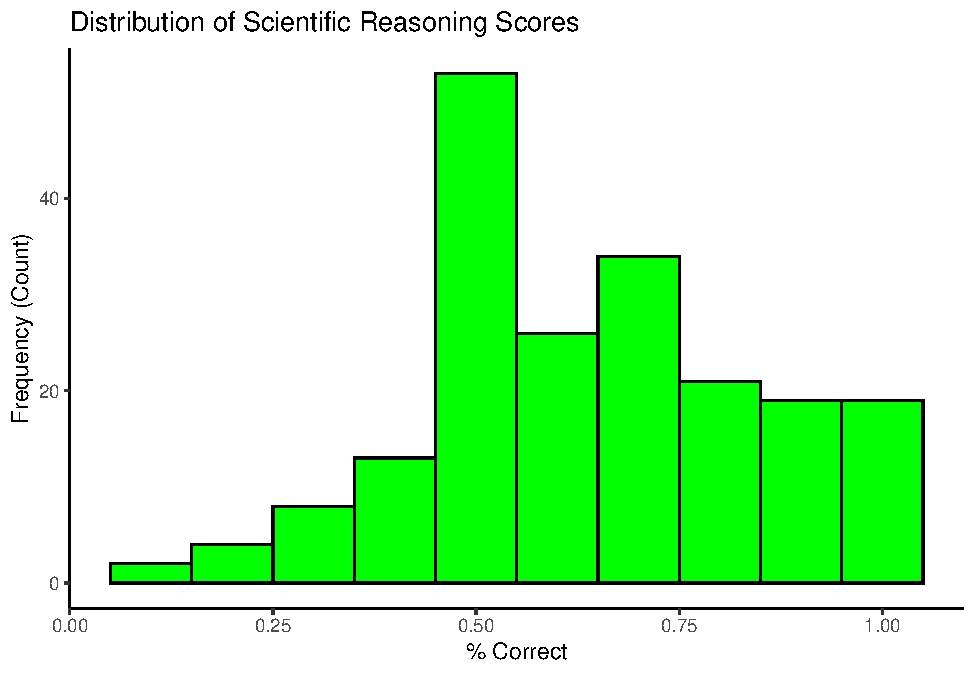
\includegraphics[keepaspectratio]{traits_reasoning_report_papaja_2025-10-26_files/figure-latex/histogram-1.pdf}}

\section{Discussion}\label{discussion}

The purpose of the present study was to examine how personality traits are related to scientific reasoning.

Overall, it seems that people reason about science, but maybe not as much as we would have hope.

We don;t actually know how personality traits are related to scientific reasoning, because we did not assess that. That is a limitation of the study that should guide future work.

In sum, this was a very mediocre study. We will try better in the future.

\newpage

\section{References}\label{references}

\phantomsection\label{refs}
\begin{CSLReferences}{1}{0}
\bibitem[\citeproctext]{ref-R-papaja}
Aust, F., \& Barth, M. (2025). \emph{{papaja}: {Prepare} reproducible {APA} journal articles with {R Markdown}}. \url{https://doi.org/10.32614/CRAN.package.papaja}

\bibitem[\citeproctext]{ref-R-tinylabels}
Barth, M. (2025). \emph{{tinylabels}: Lightweight variable labels}. \url{https://doi.org/10.32614/CRAN.package.tinylabels}

\bibitem[\citeproctext]{ref-R-labelled}
Larmarange, J. (2025). \emph{Labelled: Manipulating labelled data}. Retrieved from \url{https://CRAN.R-project.org/package=labelled}

\bibitem[\citeproctext]{ref-R-base}
R Core Team. (2024). \emph{R: A language and environment for statistical computing}. Vienna, Austria: R Foundation for Statistical Computing. Retrieved from \url{https://www.R-project.org/}

\bibitem[\citeproctext]{ref-R-groundhog}
Simonsohn, U., \& Gruson, H. (2025). \emph{Groundhog: Version-control for CRAN, GitHub, and GitLab packages}. Retrieved from \url{https://CRAN.R-project.org/package=groundhog}

\bibitem[\citeproctext]{ref-R-ggplot2}
Wickham, H. (2016). \emph{ggplot2: Elegant graphics for data analysis}. Springer-Verlag New York. Retrieved from \url{https://ggplot2.tidyverse.org}

\bibitem[\citeproctext]{ref-R-dplyr}
Wickham, H., François, R., Henry, L., Müller, K., \& Vaughan, D. (2023). \emph{Dplyr: A grammar of data manipulation}. Retrieved from \url{https://CRAN.R-project.org/package=dplyr}

\bibitem[\citeproctext]{ref-R-psych}
William Revelle. (2025). \emph{Psych: Procedures for psychological, psychometric, and personality research}. Evanston, Illinois: Northwestern University. Retrieved from \url{https://CRAN.R-project.org/package=psych}

\bibitem[\citeproctext]{ref-R-knitr}
Xie, Y. (2015). \emph{Dynamic documents with {R} and knitr} (2nd ed.). Boca Raton, Florida: Chapman; Hall/CRC. Retrieved from \url{https://yihui.org/knitr/}

\end{CSLReferences}


\end{document}
